\section{Decision Tree, Ensamble Methods \& Random Forest}
\subsection{Decision Tree}
\begin{itemize}
    \item A flow-chart-like tree structure
    \item Internal node denotes a test on a attribute
    \item Branch represent an outcome of the test
    \item Leaf nodes represent class labels or class distribution
\end{itemize}
Gini Index:
\[
I_G = 1- \sum_{j = 1}^{c}p_j^2
\]
Entropy:
\[
I_H = - \sum_{j = 1}^{c} p_j \log(p_j)
\]
\(p_j\) is the proportion of samples that belongs to calss \(j\).
Tree construction:
\begin{enumerate}
    \item Initialization: whole region \(R_0\)(i.e., all given data)
    \item Repeat:
    \begin{itemize} 
        \item For each region \(R_i\), for each feature \(X_j\), for each split \(R_i = R_{i,l} \cup R_{i,r}\) with respect to feature \(x_j\). Calculate change in impurity score (e.g., gini, entropy, error)
        \item Choose best split,i.e., maximum decrease of the impurity score
        \item Replace \(R_i\) with the two new split regions
    \end{itemize}
\end{enumerate}
Avoiding overfitting:
\begin{itemize}
    \item Select a proper depth of the tree
    \item Select a proper minimum number of samples in a leaf to stop further splitting
    \item Tree pruning - remove split nodes bottom up or top down
\end{itemize}
All these performed using either a validation set or cross validation!

\subsection{Pros/Cons}
Pros:
\begin{itemize}
    \item Easily visualized and interpreted
    \item No feature normalization or scaling needed
    \item Works well with mixed feature data types (categorical, continuous)
\end{itemize}
Cons:
\begin{itemize}
    \item Easly ovefits
    \item Not robust, high variance
\end{itemize}
\subsection{Ensamble methods}
Appproach:
\begin{itemize}
    \item Suppose you have \(n\) classifier
    \item Each classifier has error rate \(e\) 
    \item Assume the classifier are independent
    \item Take Majority vote
\end{itemize}
The combined result is wrong if \(n/2\) classifiers are wrong.
According  to central limit theorem variance reduces by factor \(n\).
\subsubsection{Bagging}
\begin{figure}[!h]
    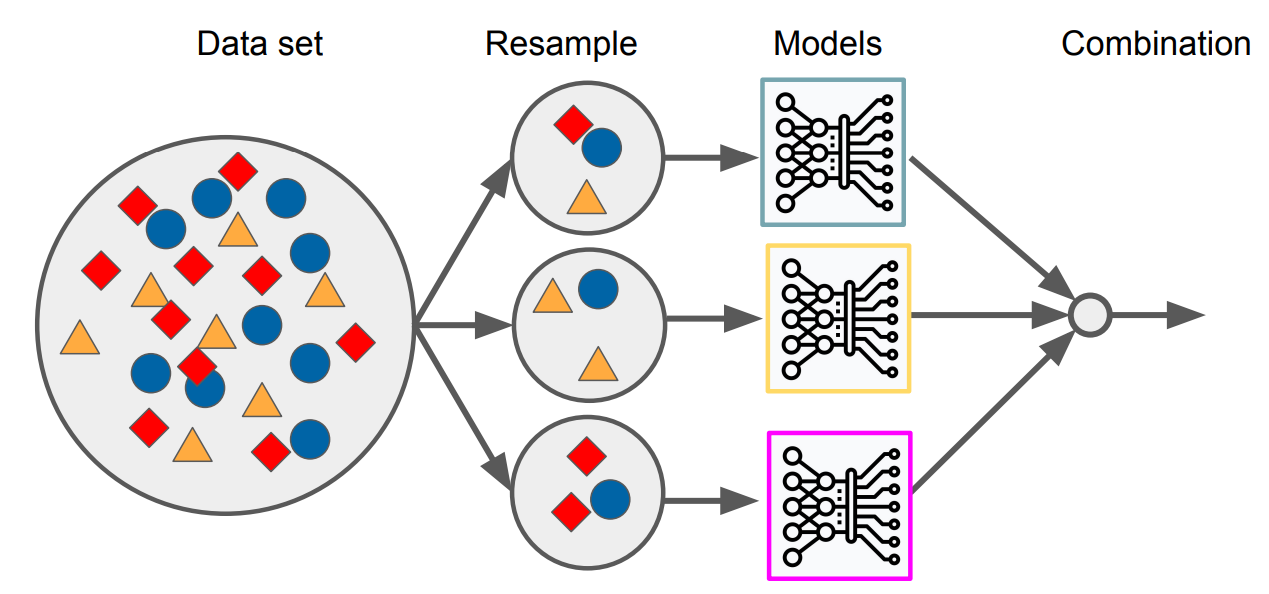
\includegraphics[width = \columnwidth]{figures/04/Bagging.png}
\end{figure}
To have independent classifier use many independent training sets \(S_i\) to train models.
\begin{itemize}
    \item Variance reduces linearly (sub-linearly in practice beacuse \(S_i\) are correlated)
    \item Bias unchanged (increases slightly in practice)
\end{itemize}

\subsubsection{Boosting}
Weight samples. Samples where the model makes mistakes are weighted higher.

Algorithm:
\begin{enumerate}
    \item Initialization: Train first model on data
    \item Repeat:
    \begin{itemize}
        \item Compute error of the model on each training sample
        \item Give higher importance to samples where the model makes mistakes
        \item Train next model using importance weighted training samples
    \end{itemize}
\end{enumerate}
In each iteration, introduce a weak model to compensate the shortcoming of the existing string (= combined) model.
\subsubsection*{Adaptive Boosting(AdaBoost)}
Take a weak learning algorithm and turn it into a strong one by making it focus more on the accurate predictions of difficult cases.
\[
F_T(x) = \sum_{t = 1}^{T}f_t(x)
\]
In each iteration \(t\):
\begin{itemize}
    \item A new weak classifier \(h(x_i)\) with a coefficant \(\alpha\) is added to the existing ones such that the error \(E_t\) of the ensemble at iteration \(t\) is minimized.
    \[
    E_t = \sum_{i}\left[F_{t-1}(x_i) + \alpha_t h(x_i)\right]
    \]
    \item The new weak classifier is training using a weighted training set where the weight assigned to each sample is identical to the error of the current ensemble classifier on that sample \(E(F_{t-1}(x_i))\).
\end{itemize}
\subsubsection{Comparison}
No Ensamble:
\begin{itemize}
    \item complete training set, train one model
\end{itemize}
Bagging:
\begin{itemize}
    \item randomly sample with replacement to obtain different training set
    \item minimizes variance (usually cannot reduce bias) -- fights overfitting
    \item Computationally efficient (all models can be trained in parallel)
\end{itemize}
Boosting:
\begin{itemize}
    \item randomly sample with replacement over weighted data to obtain different trainin sets
    \item Minimize bias by adding models to the ensemble -- fight underfitting
    \item Address variance by using simple models with low variance
\end{itemize}
\subsubsection{Random forest}
\begin{figure}[!h]
    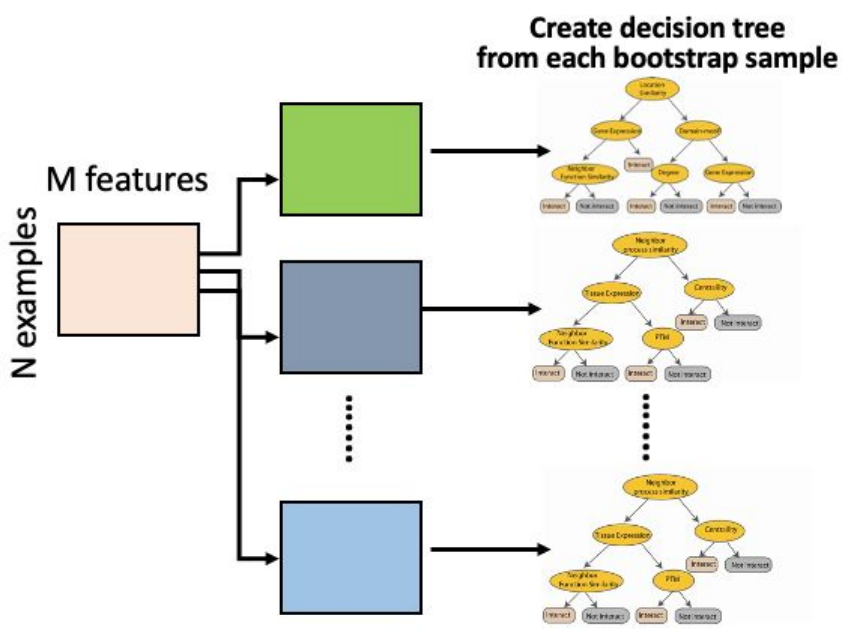
\includegraphics[width =\columnwidth]{figures/04/RandomForrest.png}
\end{figure}
Basic idea:
\begin{itemize}
    \item Grow many trees in bootstrapped samples of training data
    \item Minimize bias by growing trees sufficiently deep (overfitting)
    \item Maximize variance reduction by minimizing correlation between trees by means of bootstrapping data for each tree and sampling variable set at each node
    \item Reduce variance of noisy but unbiased trees by averaging
\end{itemize}
\subsubsection*{Out of Bag Errors (OOB Error)}
\begin{figure}[!h]
    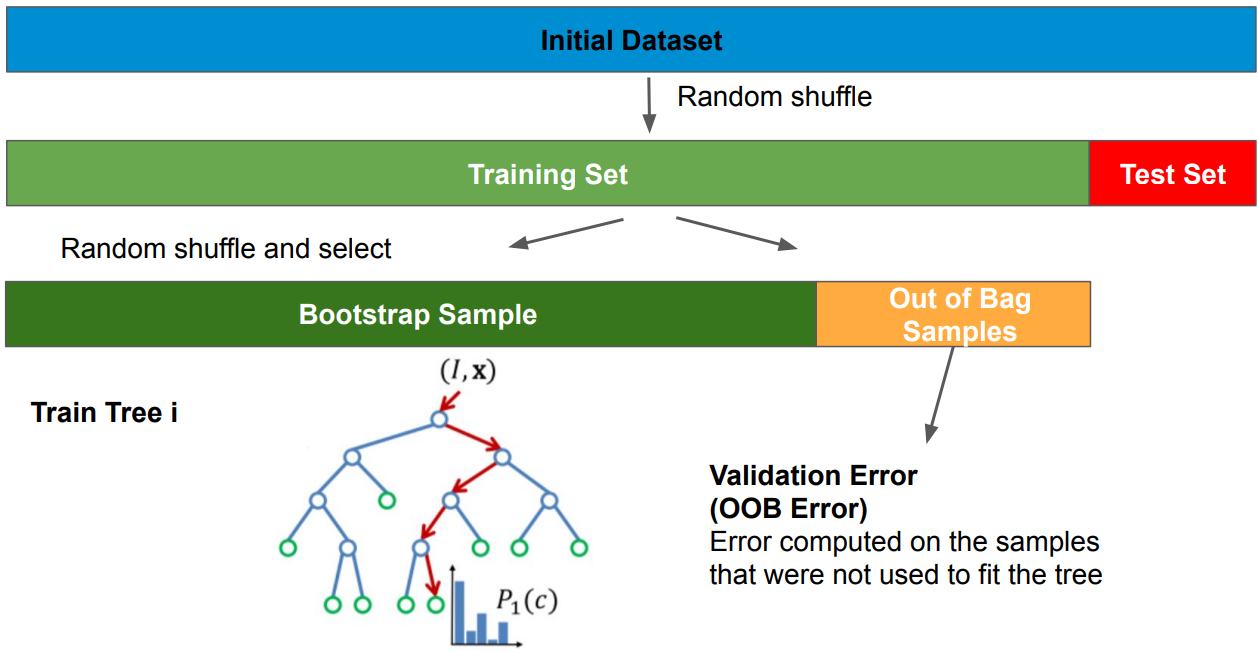
\includegraphics[width = \columnwidth]{figures/04/OOBError.png}
\end{figure}
\subsubsection{Summary Random Forrest}
Pros:
\begin{itemize}
    \item Simple - no assumption of the underlying distribution
    \item OOB error for free
    \item Many variables, even when they are not relevant for the task at hand or noisy
    \item Robust against outliers
    \item Multiclass
    \item Limit overfitting (trees have to be independent!)
    \item Unbalanced dataset (supsampling)
\end{itemize}